\documentclass[12pt]{article}
\usepackage{a4wide, amsfonts, epsfig}
\newcommand\soln{\noindent\textit{Solution:} }


%skyline stuff
\font\upright=cmu10 scaled\magstep1
\setlength{\unitlength}{0.012500in}
\begingroup\makeatletter\ifx\SetFigFont\undefined
\def\x#1#2#3#4#5#6#7\relax{\def\x{#1#2#3#4#5#6}}%
\expandafter\x\fmtname xxxxxx\relax \def\y{splain}%
\ifx\x\y   % LaTeX or SliTeX?
\gdef\SetFigFont#1#2#3{%
  \ifnum #1<17\tiny\else \ifnum #1<20\small\else
  \ifnum #1<24\normalsize\else \ifnum #1<29\large\else
  \ifnum #1<34\Large\else \ifnum #1<41\LARGE\else
     \huge\fi\fi\fi\fi\fi\fi
  \csname #3\endcsname}%
\else
\gdef\SetFigFont#1#2#3{\begingroup
  \count@#1\relax \ifnum 25<\count@\count@25\fi
  \def\x{\endgroup\@setsize\SetFigFont{#2pt}}%
  \expandafter\x
    \csname \romannumeral\the\count@ pt\expandafter\endcsname
    \csname @\romannumeral\the\count@ pt\endcsname
  \csname #3\endcsname}%
\fi
\fi\endgroup

\begin{document}
\begin{center}
{\bf 2E2 Tutorial Sheet 12 Second Term, Solutions}\footnote{Conor
Houghton, {\tt houghton@maths.tcd.ie} and {\tt
http://www.maths.tcd.ie/\char126 houghton/ 2E2.html}}
\\[1cm]
 27 January 2006
\end{center}
\textsf{
\begin{enumerate}
\item (3) Find the general solutions for the system
\begin{eqnarray}
\frac{dy_1}{dt}&=&-2y_1+y_2\\
\frac{dy_2}{dt}&=&y_1-2y_2
\end{eqnarray}
Sketch the phase diagram and and describe the node.
\vskip .5cm
\soln
This time the eigenvalues are -3 with eigenvector $\left(\begin{array}{c}-1\\1\end{array}\right)$ and -1 with  eigenvector $\left(\begin{array}{c}1\\1\end{array}\right)$. Thus,
\begin{equation}
{\bf y}=c_1\left(\begin{array}{c}-1\\1\end{array}\right)e^{-3t}+c_2\left(\begin{array}{c}1\\1\end{array}\right)e^{-t}\end{equation}
or
\begin{equation}\left(\begin{array}{c}y_1\\y_2\end{array}\right)=\left(\begin{array}{c}-c_1e^{
-3t}+c_2e^{-t}\\ c_1e^{-3t}+c_2e^{-t}\end{array}\right).\end{equation}
The phase diagram is 
\begin{center}
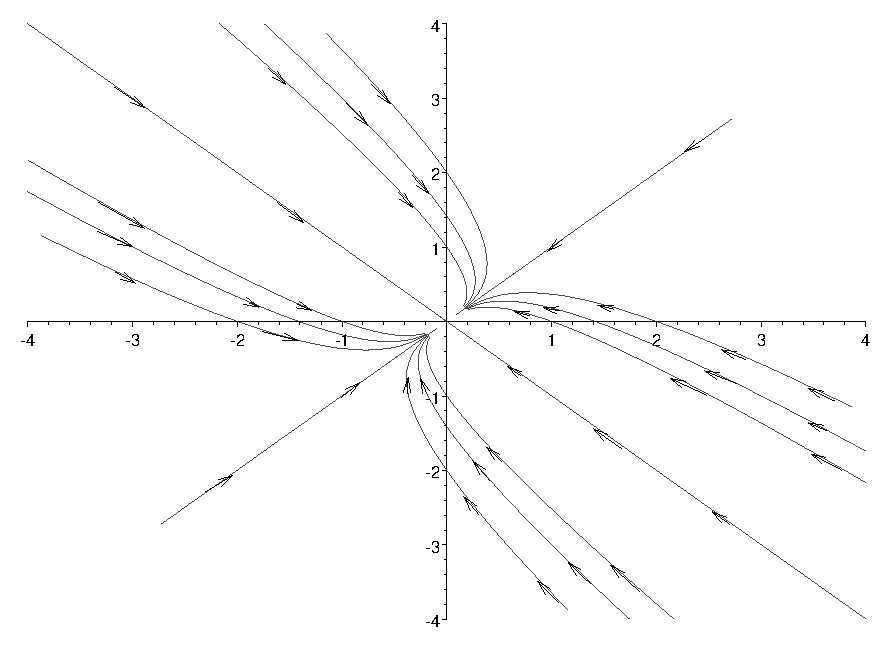
\epsfig{file=imnode.eps,
width=10cm}
\end{center}
with all the arrows pointing inwards. The node is an improper node.
\vskip .5cm
\item (3) Find the solution of 
\begin{eqnarray}
\frac{dy_1}{dt}&=&-9y_2\\
\frac{dy_2}{dt}&=&y_1
\end{eqnarray}
by considering $y_1(0)=r$ and $y_2(0)=0$, draw the phase diagram.
\vskip .5cm
\soln Working out the eigenvalues
\begin{equation}
\left|\begin{array}{cc}-\lambda&-9\\1&-\lambda\end{array}\right|=\lambda^2+9=0
\end{equation}
we find $\lambda=\pm 3i$ and the $3i$ eigenvector is 
\begin{equation}
\left(\begin{array}{cc}0&-9\\1&0\end{array}\right)\left(\begin{array}{c}a\\b\end{array}\right)=3i\left(\begin{array}{c}a\\b\end{array}\right)
\end{equation}
so $a=3i b$ and the eigenvector is, for example,
\begin{equation}
{\bf x}=\left(\begin{array}{c}3i\\1\end{array}\right)
\end{equation}
The other eigenvector is the complex conjugate of this one and so the
general solution is
\begin{equation}
{\bf
y}=c_1\left(\begin{array}{c}3i\\1\end{array}\right)e^{3it}+c_2\left(\begin{array}{c}-3i\\1\end{array}\right)e^{-3it}.
\end{equation}
\vskip .5cm
Now, if we assume that $y_1(0)=r$ and $y_2(0)=0$ we find $c_1=-c_2=-ir/6$. Putting this back in and using the sine and cosine formulas we get
\begin{equation}
{\bf y}=\left(\begin{array}{c}r\cos{3t}\\\frac{r}{3}\sin{3t}\end{array}\right)
\end{equation}
so we have the eillipse
\begin{equation}
y_1^2+(3y_2)^2=r
\end{equation}
with phase diagram
\begin{center}
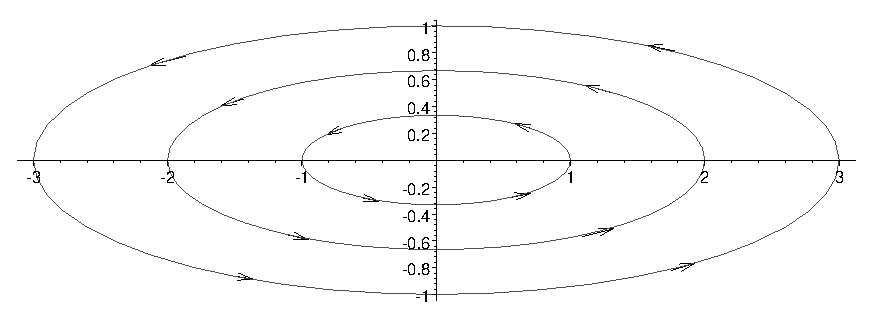
\epsfig{file=ellipses.eps, width=10cm}
\end{center}
\vskip .5cm
\item (3) Find the solution of 
\begin{eqnarray}
\frac{dy_1}{dt}&=&-y_1-2y_2\\
\frac{dy_2}{dt}&=&2y_1-y_2
\end{eqnarray}
for initial conditions $y_1(0)=r$ and $y_2(0)=0$ write this in real form. Sktech the phase diagram.
\vskip .5cm
\soln This time the matrix is 
$$A=\left(\begin{array}{cc}-1&-2\\ 2&-1\end{array}\right)$$
and so the spectrum is complex, $\lambda_1=-1+2i$ with eigenvector 
$${\bf x}_1=\left(\begin{array}{cc}i\\1\end{array}\right)$$
and $\lambda_2=-1-2i$ with eigenvector 
$${\bf x}_2=\left(\begin{array}{cc}-i\\1\end{array}\right)$$
The solution is then
$${\bf y}=\left(\begin{array}{cc}y_1\\y_2\end{array}\right)=c_1\left(\begin{array}{cc}i\\1\end{array}\right)e^{(-1+2i)t}+c_2\left(\begin{array}{cc}-i\\1\end{array}\right)e^{(-1-2i)t}.$$
Now, this means
$$
\left(\begin{array}{cc}r\\0\end{array}\right)={\bf y}(0)=c_1\left(\begin{array}{cc}i\\1\end{array}\right)+c_2\left(\begin{array}{cc}-i\\1\end{array}\right).$$
and hence $c_1=-ir/2$ and $c_2=ir/2$. Now using $\exp{(a+ib)}=\exp{a}\exp{ib}$ we have solution
$${\bf y}=\frac{r}{2}\left[\left(\begin{array}{cc}1\\-i\end{array}\right)e^{2it}+\left(\begin{array}{cc}1\\i\end{array}\right)e^{-2it}\right]e^{-t}.$$
and so
\begin{eqnarray*}
{\bf y}&=&\frac{r}{2}\left[\left(\begin{array}{cc}1\\-i\end{array}\right)(\cos{2t}+i\sin{2t})+\left(\begin{array}{cc}1\\i\end{array}\right)(\cos{2t}-i\sin{2t})\right]e^{-t}\\
&=&\left(\begin{array}{cc} r\cos{2t}\\ r\sin{2t}\end{array}\right)e^{-t}
\end{eqnarray*}
So, this gives the inward spiral. Notice how fast the spiral goes
in. The radius decreases exponentially.
\begin{center}
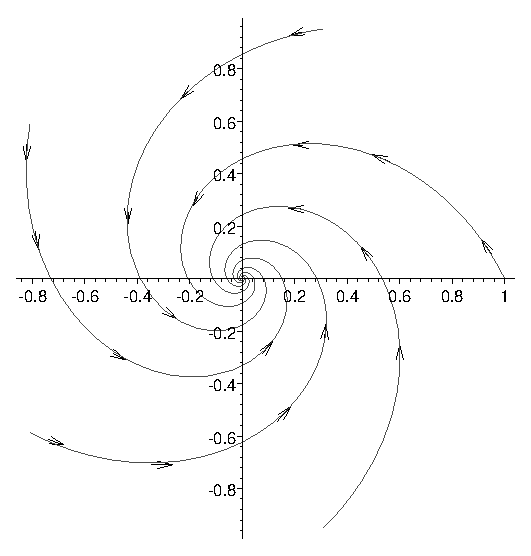
\epsfig{file=spiral.eps,width=10cm}
\end{center}
\end{enumerate}
}
\end{document}



